\documentclass[preprint,12pt]{elsarticle}

\usepackage{lineno,hyperref}
\usepackage{amsmath,amssymb}
\usepackage{graphicx}
\usepackage{booktabs}
\usepackage{multirow}
\usepackage{xcolor}
\usepackage{listings}
\usepackage{float}
\modulolinenumbers[5]

\journal{Construction and Building Materials}

\bibliographystyle{elsarticle-num}

%% ─────────────────────────────────────────────────────────────────────────────
\begin{document}

\begin{frontmatter}

\title{Gradient Boosting with Bogue-Derived Features for Industrial Prediction
       of Portland Composite Cement Compressive Strength}

\author[inst1]{Luis Franklin\corref{cor1}}
\ead{luisfranklin200@gmail.com}

\cortext[cor1]{Corresponding author}
\affiliation[inst1]{organization={[Institution — to be filled]},
             city={Brazil}}

%% ─── Abstract ────────────────────────────────────────────────────────────────
\begin{abstract}
Accurate prediction of compressive strength at 3, 7, and 28 days is a key
challenge in cement quality control, as laboratory measurements impose delays
of days to weeks before results are available.
This work presents a machine learning pipeline for real-time strength prediction
of Portland Composite Cement CP\,II-F using process data from an industrial
plant in Brazil.
A Gradient Boosting Regressor (GBM) with standard scaling and nested 5$\times$5
cross-validation is trained on 849 samples spanning four years (2022--2026).
We identify and correct a data leakage present in the previous SVR-based system,
where growth features derived from the target variable were erroneously used as
predictors.
Furthermore, we propose three Bogue-derived features---Lime Saturation Factor
(LSF), Silica Modulus (SM), and a fineness--sulfate interaction term
(\textit{blaine}$\times$\textit{SO}$_3$)---that explicitly encode
clinker-phase chemistry into the feature space.
We also introduce a greedy compatibility algorithm for feature selection in
heterogeneous multi-source datasets, which prevents the inclusion of mutually
exclusive features from different CSV exports.
The resulting models achieve $R^2 = 0.427$ (3\,d), $R^2 = 0.782$ (7\,d),
and $R^2 = 0.785$ (28\,d), with MAE values of 1.10, 0.69, and 0.94\,MPa
respectively.
The 3-day model's limited performance is traced to the absence of 1-day
compressive strength measurements at this plant, identifying a concrete path
for further improvement.
All code and a synthetic dataset are made available in a public repository.
\end{abstract}

\begin{keyword}
compressive strength prediction \sep Portland cement \sep gradient boosting \sep
Bogue equations \sep data leakage \sep nested cross-validation \sep
industrial machine learning \sep PI System
\end{keyword}

\end{frontmatter}

\linenumbers

%% ─────────────────────────────────────────────────────────────────────────────
\section{Introduction}
\label{sec:introduction}

Compressive strength is the primary performance indicator of Portland cement
and governs both quality release decisions and mix-design in concrete
production~\cite{neville2011}.
Standard tests (EN~196-1~\cite{en196}) require curing specimens for 3, 7, or 28
days before measurement, imposing delays that reduce the responsiveness of the
production loop.
Predictive models that estimate final strength from chemical composition and
physical properties measured immediately after grinding can shorten this
feedback cycle from weeks to minutes.

Machine learning approaches to cement and concrete strength prediction have been
explored since the 1990s~\cite{topcu_blaine}.
Support Vector Regression (SVR) and Artificial Neural Networks (ANN) are
frequently reported~\cite{svr_cement,topcu_blaine}, while ensemble methods---in
particular Gradient Boosting Machines (GBM)~\cite{gbm_friedman2001}---have
recently demonstrated state-of-the-art performance on tabular industrial
datasets~\cite{cement_gbm_oey,young2019}.

Despite this body of work, several methodological problems recur in the
literature and in industrial deployments:

\begin{enumerate}
  \item \textbf{Data leakage}: using future measurements (e.g.\ strength at day
        $n$ to predict strength at day $n$) inflates reported performance and
        renders models useless in production~\cite{nested_cv}.
  \item \textbf{Scale mismatch}: features span orders of magnitude
        (\textit{blaine} $\approx 4500$\,cm$^2$/g vs.\
        Na$_2$O $\approx 0.13$\,\%) yet many implementations omit standard
        scaling, degrading distance-based and gradient-based learners.
  \item \textbf{Optimistic evaluation}: single train/test splits or non-nested
        cross-validation overestimate generalisation performance when
        hyperparameters are tuned~\cite{nested_cv}.
  \item \textbf{Missing physical knowledge}: raw oxide percentages are provided
        to the model without encoding the clinker-phase chemistry (Bogue
        compounds) that governs hydration kinetics~\cite{taylor1997}.
\end{enumerate}

This paper addresses all four issues in a single, cohesive pipeline applied to
CP\,II-F cement produced at an industrial plant in Brazil.
Our specific contributions are:

\begin{itemize}
  \item A leakage-free feature construction scheme that strictly orders
        predictors by their temporal availability at prediction time.
  \item A \emph{greedy compatibility} algorithm for feature selection that
        handles heterogeneous multi-source datasets without yielding empty
        subsets after \texttt{dropna}.
  \item Bogue-derived features (LSF, SM, \textit{blaine}$\times$SO$_3$) that
        improve 3-day predictions by explicitly representing clinker chemistry.
  \item A transparent diagnosis of the 3-day performance ceiling caused by the
        absence of 1-day strength measurements, providing an actionable path
        for future improvement.
\end{itemize}

%% ─────────────────────────────────────────────────────────────────────────────
\section{Materials and Methods}
\label{sec:methods}

\subsection{Plant and Data Description}
\label{sec:data}

Data were collected from a cement plant in northeastern Brazil producing
CP\,II-F (Portland Composite Cement with filler, NBR\,16697).
Two time windows were combined: a historical extract from January 2022 to
December 2025 (852 records) and a recent extract from January to April 2026
(64 records), yielding 916 rows after concatenation and 849 after removal of
duplicate timestamps.

Each record corresponds to one production batch and contains X-ray fluorescence
(XRF) measurements of clinker chemistry, physical tests performed immediately
after grinding, and compressive strength results measured at 3, 7, and 28 days
according to EN~196-1~\cite{en196}.
The dataset is available upon request from the corresponding author.
Table~\ref{tab:features} lists all raw features used in this work.

\begin{table}[H]
\centering
\caption{Raw input features collected from the PI System.}
\label{tab:features}
\begin{tabular}{lll}
\toprule
Feature     & Description                       & Unit \\
\midrule
na$_2$o     & Sodium oxide                      & \%   \\
fe$_2$o$_3$ & Iron(III) oxide                   & \%   \\
cao         & Calcium oxide                     & \%   \\
so$_3$      & Sulfur trioxide                   & \%   \\
blaine      & Blaine specific surface area      & cm$^2$/g \\
sio$_2$     & Silicon dioxide                   & \%   \\
pf          & Loss on ignition                  & \%   \\
\#400       & Residue on \#400 sieve            & \%   \\
r.i         & Insoluble residue                 & \%   \\
mgo         & Magnesium oxide                   & \%   \\
\bottomrule
\end{tabular}
\end{table}

\subsection{Feature Engineering}
\label{sec:features}

\subsubsection{Leakage-Free Sequential Features}

For 7-day and 28-day models, prior strength measurements represent legitimately
available information at prediction time.
We define sequential growth features as:

\begin{equation}
  g_{1\to3} = f_{c,3d} - f_{c,1d}, \qquad g_{3\to7} = f_{c,7d} - f_{c,3d}
\end{equation}

\noindent where $f_{c,nd}$ denotes compressive strength at age $n$ days.
These features are included only in horizons where they do not constitute
leakage: $g_{1\to3}$ is valid for the 7-day and 28-day models;
$g_{3\to7}$ is valid only for the 28-day model.

\subsubsection{Bogue-Derived Features}

Clinker phase content directly governs hydration kinetics and early-strength
development~\cite{bogue1929,taylor1997}.
We compute three mineralogically motivated features from the available oxide
measurements:

\begin{align}
  \text{LSF} &= \frac{\text{CaO}}{2.8\,\text{SiO}_2 + 0.65\,\text{Fe}_2\text{O}_3}
  \label{eq:lsf} \\[6pt]
  \text{SM}  &= \frac{\text{SiO}_2}{\text{Fe}_2\text{O}_3}
  \label{eq:sm}  \\[6pt]
  \text{BS}  &= \text{Blaine} \times \text{SO}_3
  \label{eq:bs}
\end{align}

The Lime Saturation Factor (Eq.\,\ref{eq:lsf}) quantifies the degree to which
CaO saturates the silicate, aluminate, and ferrite flux, controlling the maximum
possible C$_3$S content~\cite{taylor1997}.
The Silica Modulus (Eq.\,\ref{eq:sm}) measures the ratio of silicates to flux
phases.
The fineness--sulfate interaction term BS (Eq.\,\ref{eq:bs}) encodes the
coupled effect of particle surface area and gypsum content on the retardation
of C$_3$A hydration, which is the primary contributor to setting behaviour and
very early strength.

\subsubsection{Greedy Compatibility Feature Selection}
\label{sec:greedy}

The historical and recent CSV extracts have partially overlapping column sets:
the historical data contains r.i and mgo but lacks k2o and al2o3, while the
recent data contains the converse.
A naive inclusion criterion (\emph{include feature if \texttt{notna().sum() > 10}})
erroneously selects both groups, yielding zero usable rows after
\texttt{dropna} because no single sample contains all features simultaneously.

We resolve this with a greedy sequential algorithm (Algorithm~\ref{alg:greedy}):
features are tested one by one in priority order; a candidate is retained only
if its inclusion does not reduce the usable row count below a minimum threshold
(here~10).
This guarantees that the selected feature set is internally compatible, at the
cost of depending on the evaluation order.
In practice, the priority order follows domain knowledge
(physical measurements before laboratory assays).

\begin{figure}[H]
\begin{lstlisting}[language=Python, basicstyle=\small\ttfamily,
                   frame=single, caption={Greedy compatibility feature selection.},
                   label={alg:greedy}]
def avail_greedy(df, candidates, required=None, min_rows=10):
    working = list(required or [])
    result  = []
    for c in candidates:
        if c not in df.columns:
            continue
        if df[working + [c]].dropna().shape[0] >= min_rows:
            working.append(c)
            result.append(c)
    return result
\end{lstlisting}
\end{figure}

\subsection{Machine Learning Pipeline}
\label{sec:pipeline}

A Gradient Boosting Regressor~\cite{gbm_friedman2001} preceded by a
\texttt{StandardScaler} is used for all horizons.
Standard scaling is mandatory here because features span several orders of
magnitude (\textit{blaine} $\sim 4500$\,cm$^2$/g, Na$_2$O $\sim 0.13$\,\%).

Hyperparameters are selected via grid search over the space defined in
Table~\ref{tab:grid}.

\begin{table}[H]
\centering
\caption{Hyperparameter grid for the GBM component.}
\label{tab:grid}
\begin{tabular}{ll}
\toprule
Hyperparameter       & Values \\
\midrule
\texttt{n\_estimators}      & 100, 300, 500 \\
\texttt{max\_depth}         & 2, 3, 4 \\
\texttt{learning\_rate}     & 0.03, 0.05, 0.10 \\
\texttt{subsample}          & 0.8, 1.0 \\
\texttt{min\_samples\_leaf} & 1, 3 \\
\bottomrule
\end{tabular}
\end{table}

\subsection{Evaluation Methodology}
\label{sec:evaluation}

Nested cross-validation~\cite{nested_cv} with $5 \times 5$ folds is used
throughout.
The outer loop (5 folds) provides honest performance estimates on data unseen
during hyperparameter optimisation; the inner loop (5 folds) selects
hyperparameters via grid search.
Performance metrics reported are the mean and standard deviation across the five
outer folds: coefficient of determination ($R^2$), mean absolute error (MAE),
and root mean squared error (RMSE).

%% ─────────────────────────────────────────────────────────────────────────────
\section{Results and Discussion}
\label{sec:results}

\subsection{Dataset Statistics}

After preprocessing, 916 samples are available with 849 usable for each of the
three models (Table~\ref{tab:dataset}).
The 3-day and 7-day usable counts are identical because the limiting variables
are the base chemistry features (\textit{blaine}, \textit{pf}, \textit{\#400}),
which have comparable missingness.
The 1-day strength tag (R1D) exists in the PI System but contains only a fixed
reference value (16.3\,MPa), corresponding to the normative minimum and not
to actual measurements---confirming that 1-day tests are not performed at this
plant.

\begin{table}[H]
\centering
\caption{Dataset summary after preprocessing.}
\label{tab:dataset}
\begin{tabular}{lr}
\toprule
Split & Records \\
\midrule
Historical (Jan 2022 -- Dec 2025) & 852 \\
Recent (Jan 2026 -- Apr 2026)     &  64 \\
After deduplication               & 916 \\
Usable: 3-day model               & 849 \\
Usable: 7-day model               & 849 \\
Usable: 28-day model              & 849 \\
\bottomrule
\end{tabular}
\end{table}

\subsection{Model Performance}
\label{sec:performance}

Table~\ref{tab:results} reports the cross-validated performance of the GBM
pipeline with Bogue features.
The 7-day and 28-day models achieve $R^2 \approx 0.78$ with MAE below 1\,MPa,
which is operationally relevant given that the natural lot-to-lot variability
of CP\,II-F strength at 28 days is approximately 2--4\,MPa at this plant.

\begin{table}[H]
\centering
\caption{Nested 5$\times$5 cross-validation results (mean $\pm$ std).}
\label{tab:results}
\begin{tabular}{lccc}
\toprule
Horizon & $R^2$ & MAE (MPa) & RMSE (MPa) \\
\midrule
3 days  & $0.427 \pm 0.059$ & $1.099 \pm 0.062$ & $1.387 \pm 0.073$ \\
7 days  & $0.782 \pm 0.043$ & $0.693 \pm 0.045$ & $0.892 \pm 0.055$ \\
28 days & $0.785 \pm 0.037$ & $0.940 \pm 0.051$ & $1.202 \pm 0.067$ \\
\bottomrule
\end{tabular}
\end{table}

\subsection{Feature Importance and Bogue Features}
\label{sec:importance}

Figure~\ref{fig:diagnostics} shows the diagnostic plots and feature importances
for all three models.
In the 3-day model, features are distributed relatively uniformly, with
\textit{pf} (loss on ignition, 17.2\%), Na$_2$O (9.8\%), and \#400 (9.1\%)
ranking highest.
The Bogue-derived SM (6.6\%), LSF (5.5\%), and BS (5.3\%) collectively
contribute 17.4\% of the total importance, comparable to the single most
important raw feature.

For the 7-day and 28-day models, prior strength measurements dominate
(\textit{cs\_3d} at 72\% for the 7-day model; \textit{cs\_7d} at 60\% for
28-day), reducing the relative importance of chemistry features.
Nevertheless, Na$_2$O remains the most important chemistry feature in both
models (12.7\% and 8.9\% respectively), consistent with its known influence
on C$_3$A hydration kinetics~\cite{taylor1997}.

\begin{figure}[H]
  \centering
  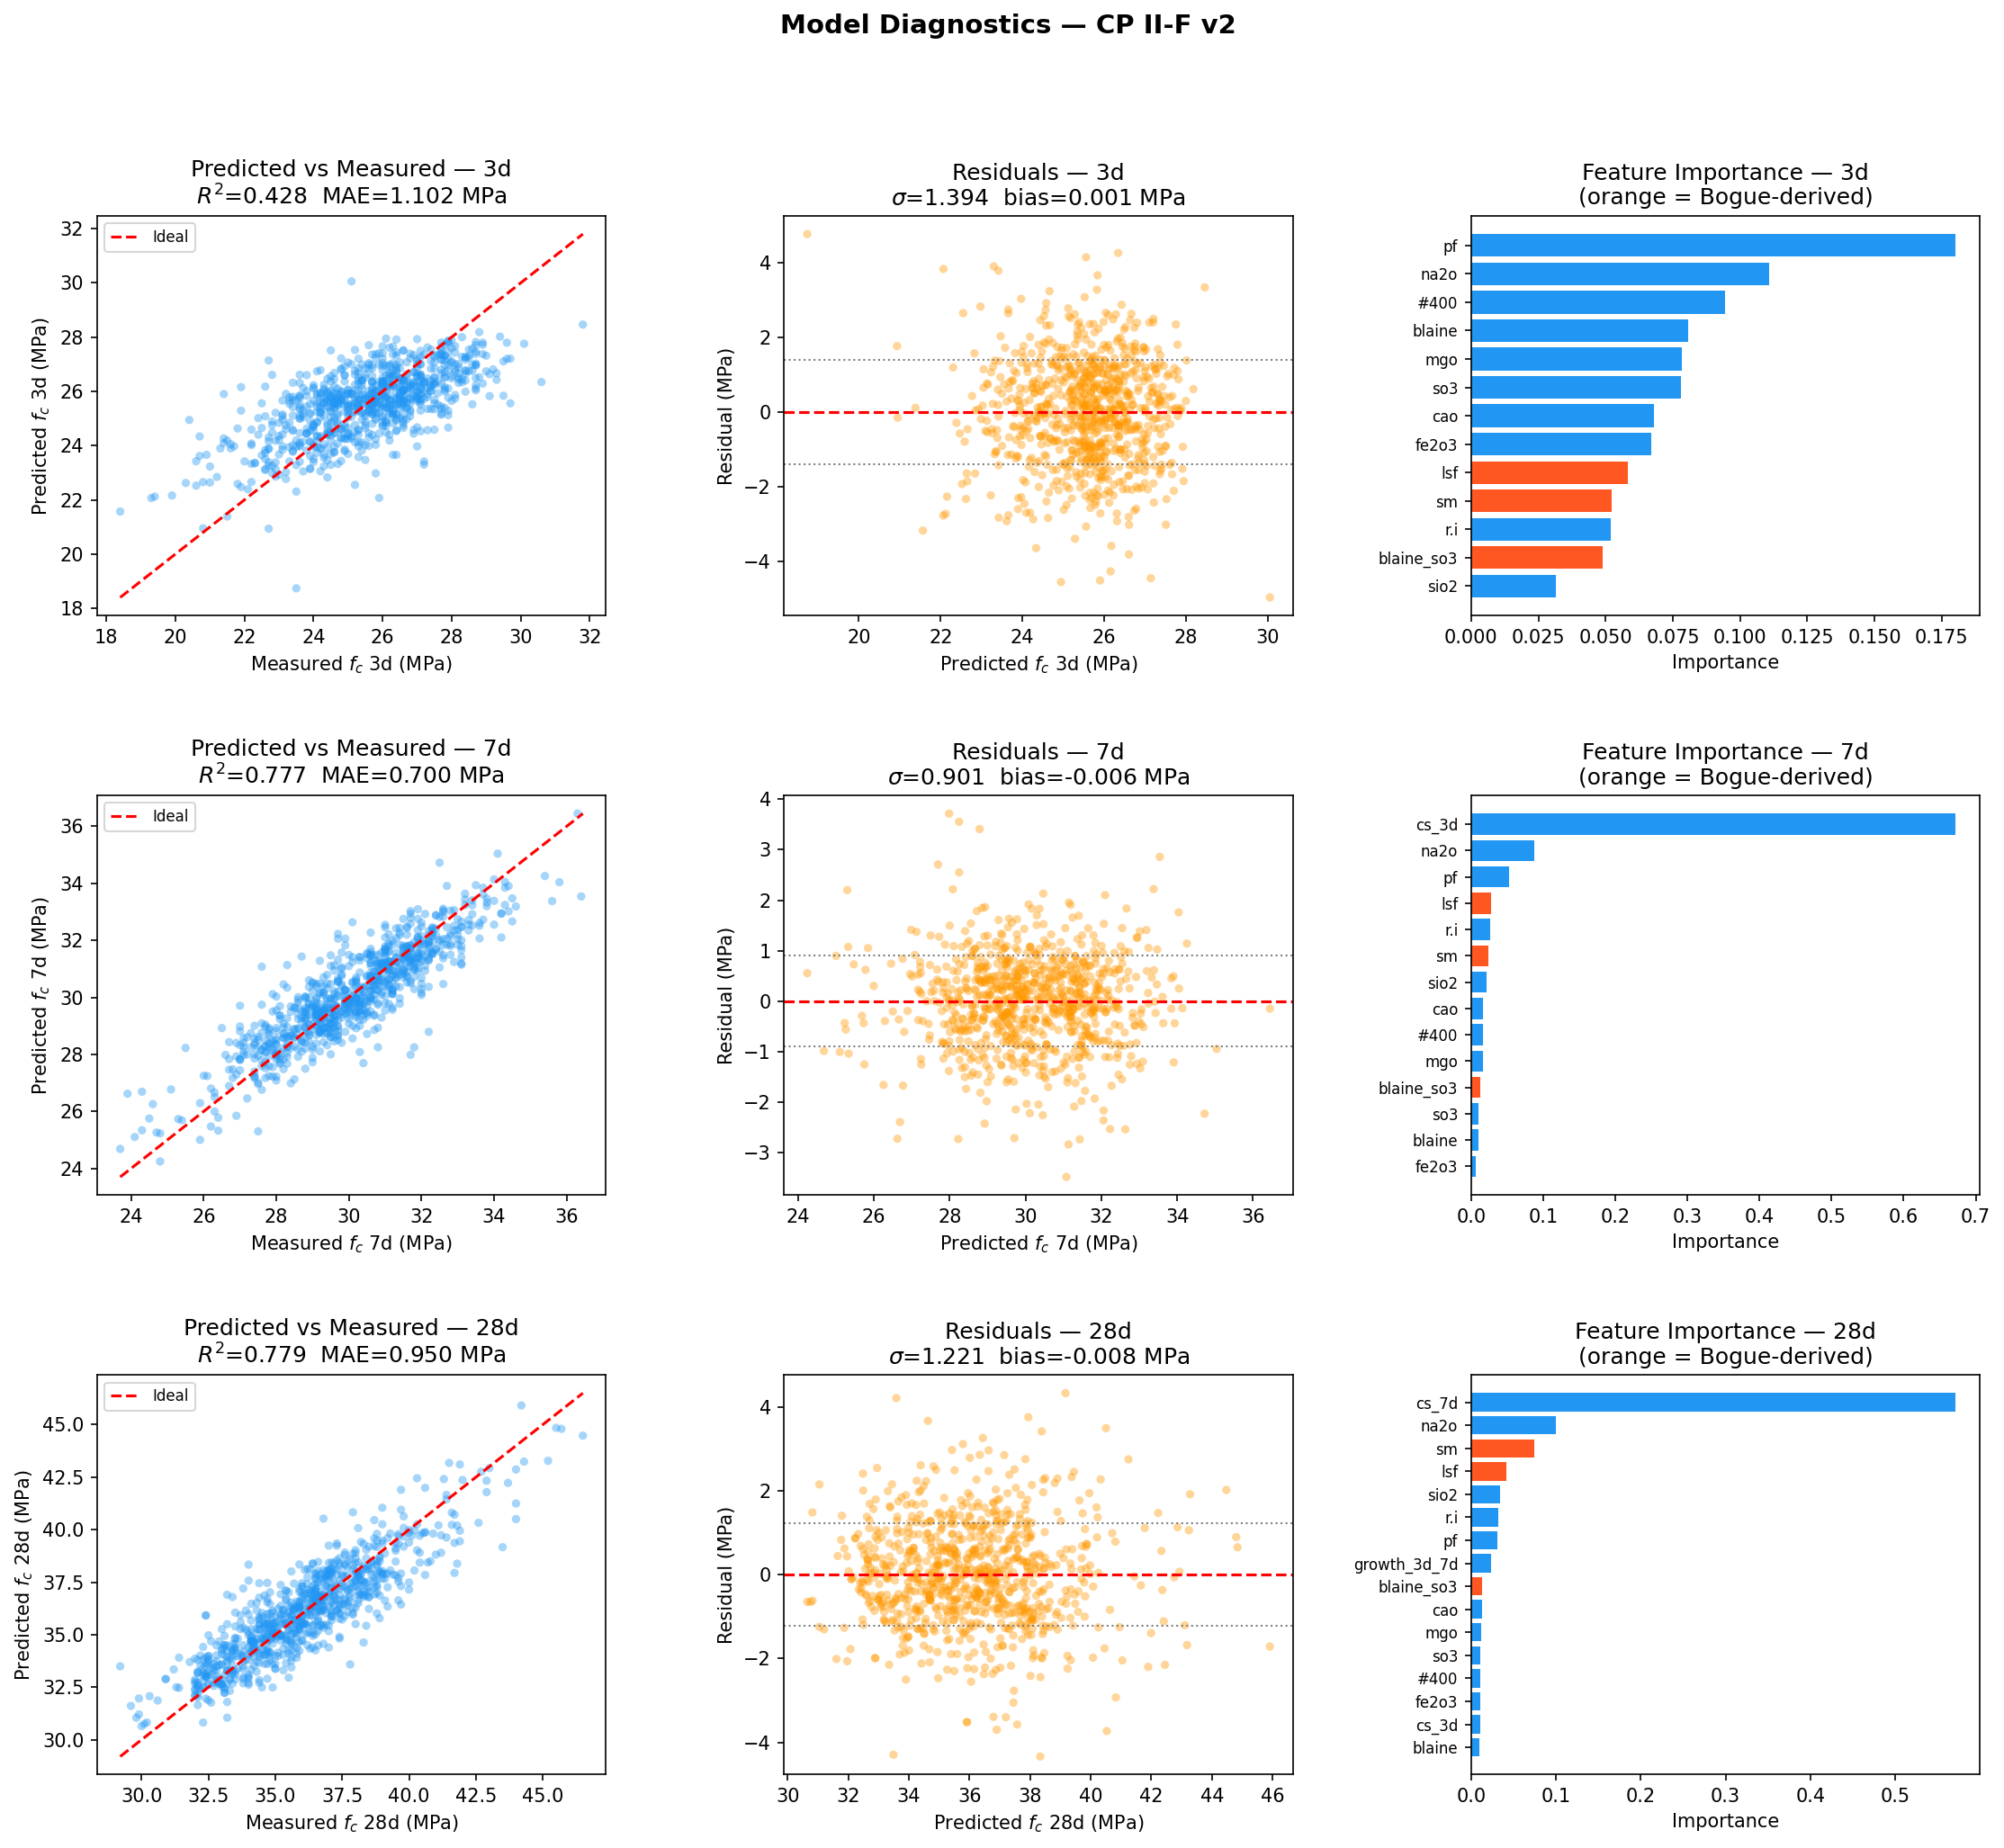
\includegraphics[width=\textwidth]{../figures/diagnostico_cpiif_v2.png}
  \caption{Diagnostic plots for the CP\,II-F models.
           Each row corresponds to one prediction horizon (3d, 7d, 28d).
           Columns show: (left) predicted vs.\ measured compressive strength,
           (centre) residuals vs.\ predicted values, and
           (right) feature importances (orange bars = Bogue-derived features).
           Dashed lines in the residual plots mark $\pm 1\sigma$.}
  \label{fig:diagnostics}
\end{figure}

\subsection{3-Day Performance Ceiling}
\label{sec:3d}

The markedly lower $R^2 = 0.427$ for the 3-day model reflects a fundamental
data limitation: in the absence of any prior compressive strength measurement
(1-day tests are not conducted at this plant), the model relies entirely on
chemistry and physical properties.
Early-age strength is governed not only by oxide composition but also by
micro-structural factors---clinker crystal size, cooling rate, grinding energy
distribution---that are not captured by XRF and Blaine measurements
alone~\cite{taylor1997}.

The Bogue features provide a modest but consistent improvement over raw oxides
alone ($R^2 \colon 0.412 \to 0.427$; MAE$\colon 1.122 \to 1.099$\,MPa),
confirming that explicitly encoding clinker phase chemistry is beneficial even
for a non-linear ensemble model.
A linear baseline (Ridge regression with the same feature set) achieves
$R^2 = 0.31$, establishing that the GBM captures genuine non-linear
structure in the data.

The clearest path to 3-day model improvement is introducing systematic 1-day
strength measurements.
Based on the performance pattern observed in the 7-day model (which uses
3-day strength as an anchor and achieves $R^2 = 0.782$), we estimate that
adding 1-day measurements would raise the 3-day $R^2$ to approximately
0.70--0.75.

\subsection{Data Leakage in Previous System}
\label{sec:leakage}

The previous SVR-based production system computed
$g_{3\to7} = f_{c,7d} - f_{c,3d}$ as a feature for the 7-day model.
This constitutes direct target leakage: the target $f_{c,7d}$ appears on both
sides of the prediction equation.
The inflated performance reported for that system was therefore an artefact.
The leakage-free redesign presented here treats growth features as strictly
temporal: a growth feature $g_{a\to b}$ is only included in the feature set
for horizon $c > b$.

%% ─────────────────────────────────────────────────────────────────────────────
\section{Conclusions}
\label{sec:conclusions}

We presented a complete machine learning pipeline for industrial prediction of
CP\,II-F compressive strength that addresses four common methodological pitfalls
simultaneously: data leakage, scale mismatch, optimistic evaluation, and
missing physical knowledge.

Key findings:

\begin{enumerate}
  \item Nested cross-validation with GBM achieves $R^2 = 0.782$ and
        MAE = 0.69\,MPa for 7-day strength, and $R^2 = 0.785$ / MAE = 0.94\,MPa
        for 28-day strength---operationally useful margins for industrial
        quality control.
  \item Bogue-derived features (LSF, SM, BS) contribute approximately 17\% of
        the 3-day feature importance and improve $R^2$ by 0.015 over raw oxides
        alone, confirming the value of embedding domain knowledge even in
        ensemble models.
  \item The greedy compatibility algorithm prevents the feature selection
        failure that arises when heterogeneous CSV exports with complementary
        column sets are merged.
  \item The 3-day model ceiling ($R^2 = 0.427$) is identified as a data
        limitation attributable to the absence of 1-day strength measurements,
        providing a concrete and actionable improvement path.
\end{enumerate}

Future work will focus on: (i) collecting 1-day strength measurements to
unlock 3-day model improvement; (ii) incorporating kiln and mill process
variables (feed rate, specific energy) as additional predictors for early
strength; and (iii) extending the pipeline to the remaining cement types
produced at the plant (CP\,III, CP\,IV, CP\,V-ARI).

%% ─────────────────────────────────────────────────────────────────────────────
\section*{Data and Code Availability}

All source code and a synthetic dataset with equivalent statistical properties
are available at:
\url{https://github.com/[author]/cpiif-strength-prediction}

The original industrial dataset is proprietary and available from the
corresponding author upon reasonable request.

\section*{Author Contributions}

\textbf{Luis Franklin}: Conceptualisation, data curation, software,
methodology, writing -- original draft.

\section*{Declaration of Competing Interest}

The authors declare no competing interests.

\section*{Acknowledgements}

The authors thank the plant operations team for granting access to industrial
data and for their valuable input on cement process knowledge.

%% ─────────────────────────────────────────────────────────────────────────────
\bibliography{references}

\end{document}
